\documentclass[12pt,fleqn]{article}
\usepackage{graphicx}

\title{\bf Computational Intelligence Midterm Exam}

\author{Matthew Saltz \\
        The University of Georgia \\
        Athens, Georgia 30602 U.S.A.}

\date{2013 March 8}

\begin{document}
\maketitle
\section{Shaffer's Function}
The first part of this report is concerned with various methods
used to optimize the function shown in Figure~\ref{fig:shaffer}.  This function
will be refered to as {\em Shaffer's function} for the remainder of the report.

\begin{figure}
\begin{center}
$$f(x,y) = 0.5 + \frac{(\sin{\sqrt{x^2+y^2}})^2 - 0.5}{[1.0+0.001(x^2+y^2)]^2}$$
\end{center}
\caption{A Variant of Shaffer's $f_6$ Function}
\label{fig:shaffer}
\end{figure}

\subsection{Genetic Algorithm}
First, a genetic algorithm was used to optimize Shaffer's function.  The inputs
$x$ and $y$ were represented as a length 64 bit string, where the first 32 bits
corresponded to a real number value for $x$, and the last 32 bits corresponded 
to a real number value for $y$.  Some manipulation was required to this 
representation in order to calculate the fitness (as specified in the instructions
for the midterm).  Four different variations of the algorithm were run:  One with 
standard mutation and uniform crossover, one with adaptive mutation and uniform 
crossover, one with standard mutation and adjusted uniform crossover, and one with
both adaptive mutation and also adjusted uniform crossover.

\subsubsection{Standard Mutation and Uniform Crossover}
Standard mutation was implemented such that each bit in a given member of the population
had a fixed probability of being flipped, or {\em mutated}.  Uniform crossover
is a bit-by-bit technique as well, such that the bits at a given position in the strings
of two species are swapped with a fixed probability.  These methods are commonly used for
genetic algorithms.

\subsubsection{Adaptive Mutation}
As an additional feature, adaptive mutation was implemented. Adaptive mutation means that
the probability of the mutation of a bit (the {\em mutation rate}) varies over time based
on certain factors.  In this case, the user specifies a maximum mutation rate, and a 
number of stable generations required for convergence (stable meaning that there has been
no change in the fitness of the most fit member), and the mutation rate is calculated 
based on these factors, along with the current number of stable generations
(Figure~\ref{fig:adaptiveMut}). Thus, the mutation rate starts at 0 and increases if there
is no change in the maximum fitness value at the end of a generation.  It continues to
increase until there is a change in the max fitness value, and then it resets to 0.  Thus,
the mutation is applied more forcefully as the GA becomes more dedicated to a given 
solution.  This also allows crossover to be effective in the earliest stages.

\subsubsection{Adjusted Uniform Crossover}
Because we are dealing with a bit string that represents real numbers, when the string
is divided into its two component parts ($x$ and $y$), a change in the bits on the left
part of each component has a much greater effect than a change in the bits on the right
part of each component.  Thus, it makes sense to design a scheme that causes crossover
to occur less frequently in the bits on the left side of each gene.  To do this, the 
probability of crossover for a bit is given by an equation relating to the bit's index
in the string (Figure~\ref{fig:adjCrossover}). In this equation, $i$ corresponds to the
bit's position in the string (with the leftmost bit having position 0). (Note: This is
applied to the $x$ and $y$ components separately).

\begin{figure}
\begin{center}
$$mutation\ rate = max\ mutation\ rate * \frac{number\ of\ stable\ generations}{stable\ generations\ for\ convergence}$$
\end{center}
\caption{Adaptive Mutation Function}
\label{fig:adaptiveMut}
\end{figure}

\begin{figure}
\begin{center}
$$crossover\_rate(i) = \frac{2^i}{2^{string\_length}}$$
\end{center}
\caption{Adjusted Uniform Crossover}
\label{fig:adjCrossover}
\end{figure}

\subsection{Particle Swarm Optimization}
Particle swarm optimization was also used to optimize Shaffer's function.  The standard
binary update equations were used, with a sigmoid function used to calculate the 
probability of a bit gaining a value of 0 or 1 based on the velocity of that dimension. A non-traditional update technique was also tried, such that $x_{new} = \lfloor v_{new}\rfloor$ $mod$ $2$ for each dimension.  Both methods were effective, with each finding the same maximum fitness value after their respective trials.

\subsection{Results}
All methods described except for the standard GA were able to find the same maximum
fitness value of 0.9975441418285032, though the $x$ and $y$ values found differed for each
method. The classic version of the PSO algorithm found this same max fitness, while the modified version was very close. All variations of the GA were run with tournament selection, a population size of 5000, and 500 generations requred for convergence.  For the runs with adaptive mutation, a maximum mutation probability of 10\% was used.  For the runs without adjusted crossover, the crossover rate was set to 50\%. Results can be
seen in figures~\ref{fig:gaResults},~\ref{fig:gaChart}, and ~\ref{fig:psoResults}.  
\begin{figure}
{\tiny
\begin{center}
    \begin{tabular}{ | l | l | l | l |}
        \hline
        Features & Fitness & x & y \\ \hline
        Standard & 0.9975441418284994 & 1.5596631907613698 & 0.17302040410528718 \\ \hline
        Adjusted Crossover Only & 0.9975441418285032 & -0.17259125056058622 & -1.5597108744885588 \\ \hline
        Adaptive Mutation Only & 0.9975441418285032 & 1.5688184663816571 & -0.03597737216409769 \\ \hline
        Both & 0.9975441418285032 & -0.03597737216409769 & -1.5688184663816571 \\ \hline
    \end{tabular}
\end{center}
}
\caption{GA Results}
\label{fig:gaResults}
\end{figure}

\begin{figure}[h]
    \centering
    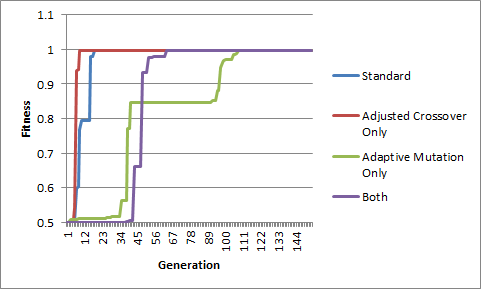
\includegraphics[width=0.9\textwidth]{./GAChart}
    \caption{Fitness over Time for Various GA Feature Sets}
    \label{fig:gaChart}
\end{figure}

\begin{figure}
{\small
\begin{center}
    \begin{tabular}{ | l | l | l | l |}
        \hline
        Features & Fitness & x & y \\ \hline
        Standard & 0.9975441418285032 & 0.17259125056058622 & 1.5597108744885588 \\ \hline
        Modified Update & 0.9975441418285022 & 0.10421278577155135  & 1.5657667078415614 \\ \hline
    \end{tabular}
\end{center}
}
\caption{PSO Results}
\label{fig:psoResults}
\end{figure}

\section{Temperature Prediction with Neural Networks}
The goal of this portion of the exam is to compare the prediction capabilities of a neural
network with two outputs versus two neural networks with one output each (the outputs
correspond to the same factors.  In this case, we are attempting to predict the
temperature 3 days and 5 days in advance, given temperature data from 4 days prior until
the current day.  We want to know if having a distinct NN to predict each factor will
produce better results than having a single network to produce both outputs. For each 
experiment, the training set consisted of 80\% of the data available, and the network's
generalization capabilities were tested on the remaining 20\% of the data as a test
set. The networks were trained until the average error in the test set was less than 0.0002 or until 20,000 learning events had occured since the last minimum average error. Each network utilized one hidden layer.  They were each trained with 81 hidden nodes.  The dual network was also trained with 161 nodes, with a negligible difference.  As you can see in the results, the minimum errors achieved for the dual and the single networks were
very similar.  However, the dual network finished training after around 40 epochs, whereas
the single networks finished around 130 epochs.  Overall, the results were very similar. It makes sense that with so few inputs and a large number of hidden nodes in comparison,
a single network could predict the temperatures just as accurately as two dedicated networks.

\begin{figure}
{\small
\begin{center}
    \begin{tabular}{ | l | l | l | }
        \hline
        Network Type &  Mean Squared Error & Max Absolute Error \\ \hline
        T3 Single Network & 0.002 & 0.368 \\ \hline
        T5 Single Network & 0.002 & 0.374 \\ \hline
        T3 Dual Network & 0.002  & 0.368 \\ \hline
        T5 Dual Network & 0.002  & 0.372 \\ \hline
    \end{tabular}
\end{center}
}
\caption{Neural Network Training Results}
\label{fig:psoResults}
\end{figure}

\end{document}
